\documentclass[tikz,border=10pt]{standalone}
\usepackage[T1]{fontenc}
\usepackage{mathpazo}
\usepackage{amsmath,amssymb}
\usetikzlibrary{arrows.meta, positioning, calc, fit}

\definecolor{stblue}{HTML}{7B97AD}
\definecolor{rwgold}{HTML}{B8995E}
\definecolor{sage}{HTML}{7A9A7E}
\definecolor{dkbrown}{HTML}{3D3530}
\definecolor{wmgray}{HTML}{7B7067}
\definecolor{cream}{HTML}{F9F6F0}
\definecolor{border}{HTML}{D4C9B8}

\begin{document}
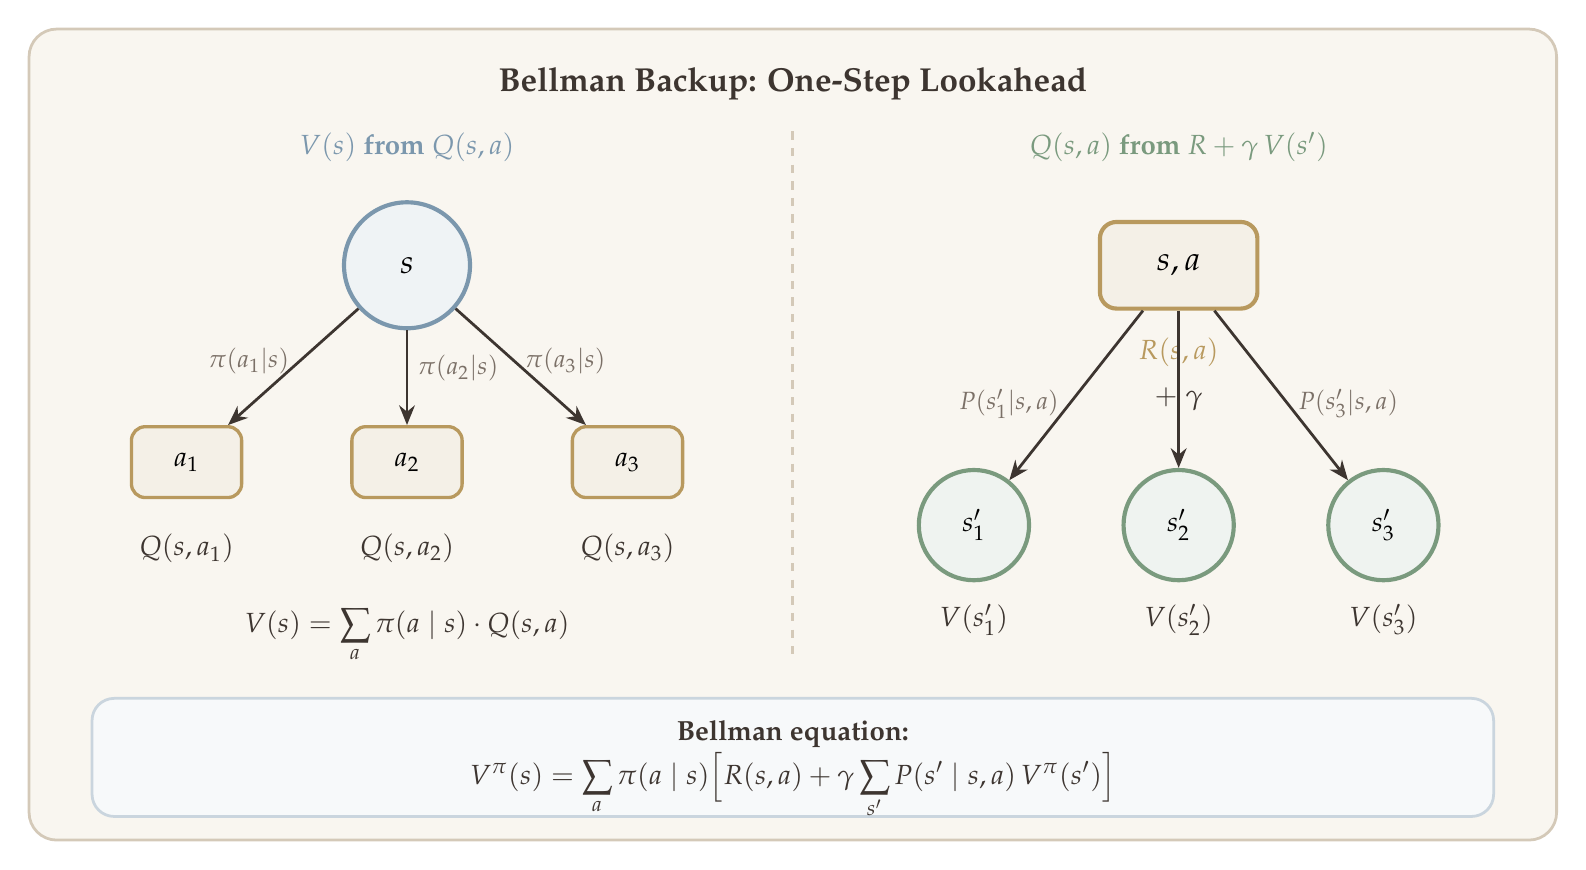
\begin{tikzpicture}[
  >={Stealth[length=2.5mm, width=2mm]},
  arr/.style={draw=dkbrown, line width=0.8pt, ->},
  snode/.style={circle, draw=stblue, line width=1.5pt, fill=stblue!12,
    minimum size=16mm, font=\large\bfseries, inner sep=0pt},
  anode/.style={rectangle, rounded corners=5pt, draw=rwgold, line width=1.2pt,
    fill=rwgold!15, minimum height=9mm, minimum width=14mm,
    inner sep=3pt, font=\normalsize\bfseries},
  spnode/.style={circle, draw=sage, line width=1.5pt, fill=sage!12,
    minimum size=14mm, font=\normalsize\bfseries, inner sep=0pt},
  sanode/.style={rectangle, rounded corners=6pt, draw=rwgold, line width=1.5pt,
    fill=rwgold!15, minimum height=11mm, minimum width=20mm,
    inner sep=3pt, font=\large\bfseries},
  elabel/.style={font=\small, text=wmgray},
]

% Background
\fill[cream, rounded corners=10pt] (-3.8,-6.8) rectangle (15.6,3.5);
\draw[border, rounded corners=10pt, line width=1pt] (-3.8,-6.8) rectangle (15.6,3.5);

% Title
\node[font=\large\bfseries, text=dkbrown] at (5.9,2.8) {Bellman Backup: One-Step Lookahead};

% Divider
\draw[border, line width=1pt, dashed] (5.9,2.2) -- (5.9,-4.5);

% ===================================================================
% LEFT SIDE: V(s) from Q(s,a)
% ===================================================================

\node[font=\normalsize\bfseries, text=stblue] at (1.0,2.0) {$V(s)$ from $Q(s,a)$};

% State s at top
\node[snode] (s) at (1.0,0.5) {$s$};

% Action nodes
\node[anode] (a1) at (-1.8,-2.0) {$a_1$};
\node[anode] (a2) at (1.0,-2.0) {$a_2$};
\node[anode] (a3) at (3.8,-2.0) {$a_3$};

% Edges from s to actions with policy weights
\draw[arr, line width=1pt] (s) -- node[elabel, left, pos=0.45] {$\pi(a_1|s)$} (a1);
\draw[arr, line width=1pt] (s) -- node[elabel, right, pos=0.4] {$\pi(a_2|s)$} (a2);
\draw[arr, line width=1pt] (s) -- node[elabel, right, pos=0.45] {$\pi(a_3|s)$} (a3);

% Q-value labels below action nodes
\node[font=\normalsize, text=dkbrown] at (-1.8,-3.1) {$Q(s,a_1)$};
\node[font=\normalsize, text=dkbrown] at (1.0,-3.1) {$Q(s,a_2)$};
\node[font=\normalsize, text=dkbrown] at (3.8,-3.1) {$Q(s,a_3)$};

% Equation
\node[font=\normalsize, text=dkbrown] at (1.0,-4.2)
  {$\displaystyle V(s) = \sum_a \pi(a \mid s) \cdot Q(s,a)$};

% ===================================================================
% RIGHT SIDE: Q(s,a) from R + gamma V(s')
% ===================================================================

\node[font=\normalsize\bfseries, text=sage] at (10.8,2.0) {$Q(s,a)$ from $R + \gamma \, V(s')$};

% State-action pair at top
\node[sanode] (sa) at (10.8,0.5) {$s, a$};

% Reward + discount label
\node[font=\normalsize\bfseries, text=rwgold] at (10.8,-0.6) {$R(s,a)$};
\node[font=\normalsize, text=dkbrown] at (10.8,-1.2) {$+ \;\gamma$};

% Next states
\node[spnode] (sp1) at (8.2,-2.8) {$s'_1$};
\node[spnode] (sp2) at (10.8,-2.8) {$s'_2$};
\node[spnode] (sp3) at (13.4,-2.8) {$s'_3$};

% Edges from (s,a) to next states with transition probabilities
\draw[arr, line width=1pt] (sa) -- node[elabel, left, pos=0.55] {$P(s'_1|s,a)$} (sp1);
\draw[arr, line width=1pt] (sa) -- (sp2);
\draw[arr, line width=1pt] (sa) -- node[elabel, right, pos=0.55] {$P(s'_3|s,a)$} (sp3);

% V(s') labels below next states
\node[font=\normalsize, text=dkbrown] at (8.2,-4.0) {$V(s'_1)$};
\node[font=\normalsize, text=dkbrown] at (10.8,-4.0) {$V(s'_2)$};
\node[font=\normalsize, text=dkbrown] at (13.4,-4.0) {$V(s'_3)$};

% ===================================================================
% BOTTOM: Combined Bellman equation box
% ===================================================================

\draw[stblue!40, rounded corners=8pt, line width=1pt, fill=stblue!6]
  (-3.0,-6.5) rectangle (14.8,-5.0);

\node[font=\normalsize\bfseries, text=dkbrown] at (5.9,-5.45)
  {Bellman equation:};
\node[font=\normalsize, text=dkbrown] at (5.9,-6.1)
  {$\displaystyle V^\pi(s) = \sum_a \pi(a \mid s)\Bigl[R(s,a) + \gamma \sum_{s'} P(s' \mid s,a)\, V^\pi(s')\Bigr]$};

\end{tikzpicture}
\end{document}
